\documentclass[11pt]{article}

\usepackage{thumbpdf, amssymb, amsmath, amsthm, microtype,
	    graphicx, verbatim, listings, color, fancybox}
\usepackage[pdftex]{hyperref}
%\usepackage[margin=1in]{geometry}
\usepackage{cawsty}
\usepackage{fullpage}
\usepackage{pseudocode}

\usepackage{algorithm}
%\usepackage{algorithmic}
\usepackage{amsmath}
\usepackage{amsthm}
\usepackage{algpseudocode}
\usepackage{algorithmicx}% http://ctan.org/pkg/algorithmicx
\usepackage{lipsum}% http://ctan.org/pkg/lipsum
\usepackage{xifthen}% http://ctan.org/pkg/xifthen
\usepackage{needspace}% http://ctan.org/pkg/needspace
\usepackage{hyperref}% http://ctan.org/pkg/hyperref

% ================ ALGORITHM ENVIRONMENT ================
\newcounter{numberedAlg}% Algorithm counter
\newenvironment{numberedAlg}[1][]%
  {% \begin{numberedAlg}[#1]
    \needspace{2\baselineskip}% At least 2\baselineskip required, otherwise break
    \noindent \rule{\linewidth}{1pt} \endgraf% Top rule
    \refstepcounter{numberedAlg}% For correct reference of algorithm
    \centering \textsc{Algorithm}~\thenumberedAlg%
    \ifthenelse{\isempty{#1}}{}{:\ #1}% Typeset name (if provided)
  }{% \end{numberedAlg}
  \noindent \rule{\linewidth}{1pt}% Bottom rule
  }%

%\setlength{\parindent}{0pt}

\linespread{1.2}

\begin{document}
\arltitle{Engineering Networks for Optimal Robustness}{Data Communication and Networks I [4005-700]}

\begin{abstract}
Due to the growing pervasiveness of civilian and 
military networks for the transmission of safety-critical and real-time data, 
it is critically important that they are resistant to selective and random network 
node deletions. Network robustness is a measure of the performance and 
throughput responsiveness of a network in response to such deletions. The nature of 
this metrics lends itself to the application of percolation theory, which can be
used to describe the behavior of connected clusters in a random graph. This theory
can be utilized to design and construct optimally robust networks in order to yield
the best performance in the event of node deletions.

This paper presents some background information on network robustness and
its importance in modern communication systems, with a specific focus on wireless sensor networks, presents some recent advances made in the topic, and concludes with avenues of future work that can be explored by researchers in the field. 
\end{abstract}

% http://crpit.com/confpapers/CRPITV26Dekker.pdf
% http://en.wikipedia.org/wiki/Percolation_theory
% http://arxiv.org/abs/cond-mat/0007300
% http://www.research.ibm.com/people/r/rish/papers/PhysicaA_3_30.pdf
% http://www.cs.berkeley.edu/~dawnsong/papers/coloring_ndss08_cr.pdf

% robust routing and dynamic load balancing - the hw/sw solution to help deal with robustness and traffic changes
% http://iie.fing.edu.uy/investigacion/grupos/artes/publicaciones/casas_drcn09.pdf

\section{Introduction}

Military and civilian communications have seen two common trends in rencent years: an 
increase in network-oriented operations and an increase in high-risk threats to
such networks \cite{Bernard_networkrobustness}. These operational efforts place
high reliance on the underlying network infrastructure for communication, so it is vital
that this communication medium is protected against emerging attacks that focus on
specific nodes in the network or communication lines that join nodes together. In this context
the type of network attacks are irrelevant; the focus is more aligned with the optimal topology
of networks and technological aids that can be utilized to help handle any changes in this topology. 

This focus can be seen by a significant increase in research oriented around robust network design that provides high throughput and connectivitiy among all nodes in the network, especially when specific nodes are intentionally or unintentionally deleted from the network. Subsequently, the robustness of such networks can be viewed as a qualitative or quantitative measure of the network's resilience to such topology changes.

The problem of designing such networks has lent itself as a useful application of both graph theory and percolation theory. Graph theory has been applied to mathematically analyze the robustness of networks represented as undirected graphs based on their levels of vertex and edge connectivity. Similarly, percolation theory has been applied to study the behavior of connected clusters in undirected network graphs. 

This paper will focus on recent research efforts centered around both of these branches of 
mathematical theory and their application to network design. It will also present practical methods of
network engineering that have been employed to help networks deal with topology changes dynamically.
Lastly, it will discuss avenues for future research and open problems that have been posed by 
researchers in the field.

\section{Fundamentals}

It is natural to model any communication network as an undirected graph $G$, which has a fixed 
set of vertices (nodes) $V(G)$ and edges (links) $E(G)$ that represent physical connections between such vertices. For conveniene, we let $N = |V(G)|$ and $M = |E(G)|$. The topology of a network
can thus be visualized graphically using elements from these two sets. For the remainder of this paper,
we use the term vertex as a synonom for node and edge as a synonom for communication link. As an example of a graph representing a network, consider a completely connected network with $n$ nodes in which every node can directly communicate with every other 
node can be seen as $K_{n}$, the complete graph on $n$ vertices (that is, $|V(G)|$ $= n$). In such a network, every node $v$ can
communicate with exactly $n-1$ other nodes, which means that its degree $deg(v) = n-1$. 

In order to discuss the connectivity of networks, it is necessary to define the connectivity of such
graphs in terms of both the vertices and edges. We introduce the following terms to use throughout 
the remainder of this paper.

% graph connectivity
\begin{define}
A graph $G$ is said to be \textbf{connected} if and only if $\forall u,v \in V(G)$ there exists a path between $u$ and $v$.
\end{define}

% graph, vertex, edge, degree,
% path
% vertex connectivity
% edge connectivity
% component

\section{Network Functionality}
\label{NetworkFunctionality}

Network engineers strive for high performance networks that exhibit high throughput and low 
latency between any two nodes in the same network. Several mathematical metrics based on
the corresponding graph that represents a network have been proposed to reflect this need. 
For example, metrics such as the average geodesic path length between any two nodes in a network, which equates to the average shortest path) and vertex and edge betweeness (which are essentially measures of centralities located within a graph). 

The average geodesic length $L$ can be defined as follows,
\begin{eqnarray*}
L(d(v,w)) = \frac{1}{N(N-1)}\sum_{v \in V(G)}\sum_{w \not= v \in V(G)} d(v,w),
\end{eqnarray*}
where $d(v,w)$ is the distance of the shortest path between vertices $v$ and $w$, and $N(N-1)$ is the total number of pairs of vertices, independent of whether or not each pair represents an edge in $E(G)$. The most immediate result from this measurement is that large values for $L$ indicate that the average length between any two nodes in the network is long, and thus the latency between two nodes will be proportionally large as well. 

Another important metric that measures the functionality of a network is the measure of vertex and edge centrality in the network. Although a high measure of centrality may indicate more traffic funnels through a vertex or an edge, it also implies that any attacks on this vertex or edge would most likely have an negative impact on the traffic in the network by increasing the load on neighboring nodes and increasing the average geodesic path length. Although there is not a single definition for this metric, Holme et al \cite{Attacks} propose the use of the following definitions for vertex, $C_{B}(v)$ and edge $C_{B}(e)$ centrality.
\begin{eqnarray*}
C_{B}(v) = \sum_{w \not= x \in V(G)} \frac{\sigma_{wx}(v)}{\sigma_{wx}},
\end{eqnarray*}
where $\sigma_{wx}(v)$ is the number of paths between $w$ and $x$ that pass through $v$ and $\sigma_{wx}$ is total of paths from $w$ to $x$ (notice that $\sigma_{wx}(v) \leq \sigma_{wx}$).
\begin{eqnarray*}
C_{B}(v) = \sum_{w \not= x \in V(G)} \frac{\sigma_{wx}(e)}{\sigma_{wx}}
\end{eqnarray*}
As in the centrality measure for vertices, $\sigma_{wx}(e)$ is the number of paths between $w$ and $x$ that contain $e$ and $\sigma_{wx}$ is total of paths from $w$ to $x$ (notice again that $\sigma_{wx}(e) \leq \sigma_{wx}$).

It is important to note that the centrality of a vertex and its measure of centrality are not the same metrics. In fact, as will be shown in section~\ref{AttackStrategies}, network attacks can vary based on the measure an adversary is trying to reduce. 

Finally, we introduce a metric that characterizes the number of nodes (or rather, a fraction of the total nodes) that need to be removed in order for the graph to become globally disconnected. Let $G$ be a graph with $N - q$ nodes of degree $1$. Then, the fraction of total nodes $f_c$ that need to be randomly removed before total connectivity is lost consists of $q = [(\langle k \rangle - 1) / \sqrt{\langle k \rangle}]\sqrt{N}$ nodes of degree $\sqrt{\langle k \rangle N}$. 

%TODO: read http://polymer.bu.edu/hes/articles/pshs06.pdf and discuss the metric here - devote entire section to it in the NR part

%\section{Network Attacks}
%HDA - high degree adaptiveness - onion
% from: http://polymer.bu.edu/~hes/networks/hsmah11.pdf

%more from http://www.ncbi.nlm.nih.gov/pubmed/12059649
%Some other attacks are described in \cite{Attacks}

%TODO: describe some common networks here, why they are studied, etc
%TODO: depends on type of network (is it ad-hoc or fixed topology?)

\section{Attack Models}
\label{AttackStrategies}
%TODO: vertex/edge based attacks, degree or betweeness attacks
Attacks on large scale networks are not usually ad-hoc; they are based on a logical and structured strategy for dereasing the connectivity of the network by taking as little action as possible. Clearly, if one was to delete all nodes from a network, then that would yield the maximum decrease in connectivity. However, such attacks are not practical, so these strategies must be considered at a smaller scale. 

From a general perspective, practical attacks are theoretically focused on the objective of decreasing the number of total links in the network or the average geodesic length (or both). Consider, for example, the situations of cutting communication cables or performing a DDOS attack on a node or server with a high measure of centrality. Such attacks would decrease the number of edges in the network graph and increase the average geodesic path length, respectively. 

From the definitions presented in section~\ref{Definitions}, we can see that the number of edges in the network is directly related to the degree of each vertex (in fact, we know that $2|E(G)| =\sum_{v \in V(G)}deg(v)$). On the other hand, the measure of centrality of a vertex or edge is more related to the average geodesic path length in the network. As such, we consider practical attack patterns that focus on decreasing both of these measurements by targeting individual vertices and/or edges, as well as randomized attacks that have no specific targets. 

In general, most focused attacks fall under one of the following four categories \cite{Attacks}.
\begin{itemize}
	\item \textbf{ID removal} - initial degree distribution vertex/edge removal
	\item \textbf{IB removal} - initial betweenness distribution vertex/edge removal
	\item \textbf{RD removal} - recalculated degree distribution vertex/edge removal
	\item \textbf{RB removal} - recalculated betweenness distribution vertex/edge removal
\end{itemize}

\begin{figure}[h!]
	\label{fig:Onion}
	\centering
		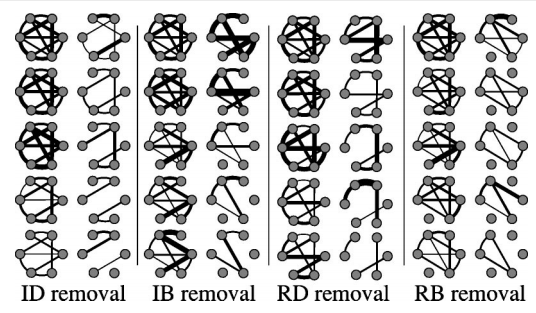
\includegraphics[width=0.5\textwidth]{edge_attacks.png}
	\caption{Various edge-centric attacks for a fixed graph structure.}
\end{figure}

RD and RB attacks on vertices yield the optimal results because they take a greedy approach to decrease the target metric. However, the implication of these attacks is that there exists an efficient and tractable way to measure these metrics after every change, which isn't always the case (especially when the topology of the network is unknown). Therefore, ID and IB attacks are more realistic, but they also assume some prior knowledge of the network infrastructure before the attack begins. Attacks that do not rely on this knowledge are referred to as random attacks, and are discussed in section~\ref{RandomFailures}.

Furthermore, it should be noted that both the ID and RD attacks are computationally less taxing than IB and RB attacks \cite{Attacks}. In fact, the time complexity of a successful ID attack (and subsequently, an entire RD attack), runs in linear time with respect to N, whereas the time complexity of betweenness-based attacks has a time complexity of $O(NL)$. The implication of this is that the adversary must make tradeoffs based on their knowledge of the network infrastructure.

\subsection{Random Failures}
\label{RandomFailures}
A common way to model attacks on a network is assume that each node and link has a fixed probability $p$ and $q$ of failing, where the exact cause of the failure is not know and is not important. Furthermore, failures are typically seen as independent events \cite{RandomStudy}. Such models are useful when analyzing complex networks such as the Internet and other related military communication networks. 

\section{Network Robustness}
%http://arxiv.org/pdf/1203.2982v1.pdf

Many different measures for network robustness have been proposed in recent years. All of which tend
to use the notion of densely connected components in the corresponding graph. In this section we present
a two unique instances of such measurements, one of which is based entirely on node topology and the other that is based on both nodes and their respective edges, and summarize their accuracy when applied to real networks.

\subsection{Robustness Measurements}
A natural way to think of network robustness is from the perspective of individual nodes, since they are 
usually the primary targets in malicious or non-malicious network attacks. Using this idea, Herrmann et al
defined a concise equation for calculating the robustness of a network based on the size of connected
components in the corresponding graph that is adapted from percolation theory. Mathematically, this can be defined as follows \cite{Onion}:
%24: http://polymer.bu.edu/~hes/networks/hsmah11.pdf
\begin{eqnarray*}
R_{n} = \frac{1}{n}\sum_{q=\frac{1}{n}}^{1}S(q)
\end{eqnarray*}
This robustness measurement computes the fractions of nodes in the largest connected cluster $S(q)$ after removing $q$ nodes. This is an intuitive calculation, since the goal of engineering robust networks is to ensure the highest measure of connectivity in the event of any node deletions. Furthermore, it has been mathematically verified to represent the exact amount of nodes that need to be deleted for the network to collapse when targeted by high-degree adaptive attacks, which are a specific class of attacks that attempt to remove highly connected nodes from the network. 

In their study of optimal graph structures that yield the highest resilience to such attacks, Herrmann et al found that most networks will exhibit onion topolgies, meaning that there are distinct layers of nodes that are connected, and that each layer $i$ has more connectivity than its parent layer $i+1$ \cite{Onion}. Another interesting property of the onion graph is that for almost every pair of vertices $u, v \in V(G)$ with the same degree, there exists a a path between $u$ and $v$ that does not contain any vertex of a higher degree. An example of such a graph with $124$ nodes and $366$ edges is shown in Figure~\ref{fig:Onion}.

\begin{figure}[h!]
	\label{fig:Onion}
	\centering
		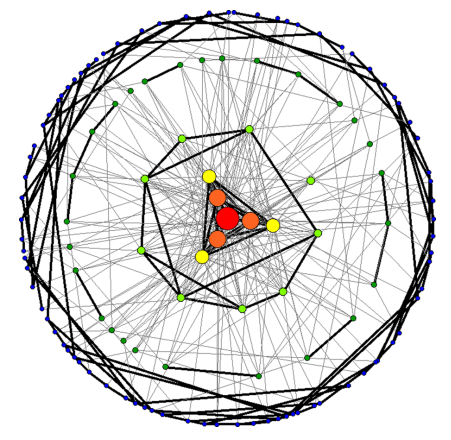
\includegraphics[width=0.5\textwidth]{Onion.jpg}
	\caption{An example of a graph with $124$ nodes and $366$ edges that exhibits the onion-like topology \cite{Onion}}
\end{figure}

Herrmann et al have also conducted research on optimization algorithms that increase this robustness measure while at the same time maintaining the distribution of vertex degrees throughout the network. Their proposed algorithm seeks to re-arrange node edges and connections to improve the resilience of the host network to any kinds of attacks using Monte-Carlo simulations. This algorithm can be described as follows:

% the re-structure algorithm
\begin{numberedAlg}[Robustness Optimization]
\label{alg1}
\begin{algorithmic}[1]
        \item Choose two random edges $(a,b)$ and $(c,d)$ from the graph $G$.
	\item Replace these edges with $(a,c)$ and $(b,d)$.
	\item If $R_{new} > R_{old}$, accept the swap and goto step 1. Otherwise, revert the swap and goto step 1. 
\end{algorithmic}
\end{numberedAlg}

Algorithm~\ref{alg1} is repeated for a very large number of iterations until an ideal level of robustness has been obtained, albiet at the sake of sometimes massive computations (as is the case with Monte-Carlo methods).

%TODO: http://arxiv.org/pdf/1203.2982v1.pdf, \cite{NRMalicious}

Another way to study the measure of robustness of a network is to examine its communication links. From the perspective of such links that exist in a network, the most successful attacks are those that take down the take down the most important or centralized communication links. As such, a common research trend has been to examine the largest components of a network with respect to the edge-betweenness, link clustering coefficient, and degree product \cite{NRMalicious}. One common measurement of the robustness of a network with respect to these metrics and the largest component of a network $S(p)$ is shown below:
\begin{eqnarray*}
R_l = \frac{1}{M}\sum_{p = 1/M}^{1}S(p)
\end{eqnarray*}
This measurement is mathematically similar to the previous node-based calculation, but instead of considering the density of the nodes in the entire component, it considers the density of the edges. 

Due to the typical attacks that are launched on networks, such as large-scale DDoS attacks that take both nodes and links to that node offline, it is natural to extend the concept of network robustness to consider both node and link failures simultaneously. However, rather because the two aforementioned measurements are based on two separate dimensions of networks, it is not simply a matter of merging them together to yield the optimum result. Instead, the measurement is typically abstracted into the context of the attack that is launched on a network, where the input parameter into the largest component is now the number of steps that have been completed at a given instance in time. Mathematically, this hybrid measurement $Q$ can be computed as follows \cite{NRMalicious}:
\begin{eqnarray*}
Q = \frac{1}{M}\sum_{step  = 1}^{M}S(step)
\end{eqnarray*}

\section{Network Topologies and Robustness Measures}
% look at: http://web.mit.edu/medard/www/rls.pdf ???

\subsection{Random Networks and Scale-Free Networks}
Following the insight that hostile vertex attacks that target important nodes with large degrees tend to cause the most significant damage to a network, Albert et al. performed extensive studies on the robustness of random and scale-free graphs. Random graphs, as the name suggests, are graphs with no specific node or edge distribution. On the other hand, scale-free graphs are special types of graphs in that the distribution of node degrees asymptotically follows a power law (i.e. $P(d) \approx d^{-\gamma}$, for some degree $k$ of a vertex $u \in V(G)$). By examining each of these classes of graphs in the context of random vertex deletions and targeted vertex attacks, it has been shown that random graphs are more robust against intentional vertex attacks, whereas the scale-free graphs are more robust against random deletions. This can be seen in Figure \ref{RandomResults}, where the breaking point of the largest component of the graphs $S$ drops off quicker for random graphs when attacked randomly \cite{GraphThesis}. 

\begin{figure}[h!]
	\label{fig:RandomResults}
	\centering
		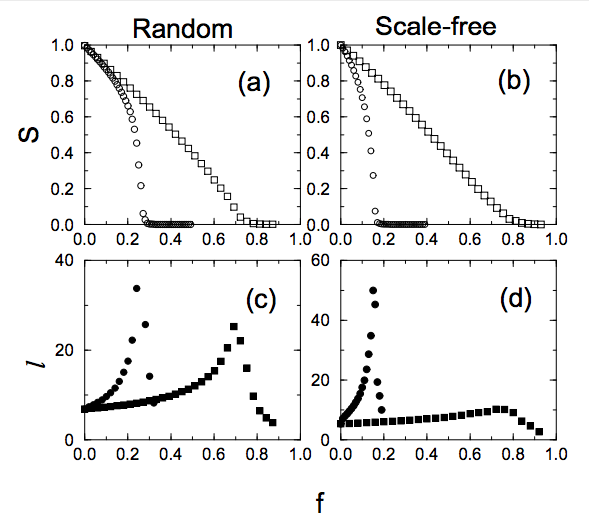
\includegraphics[width=0.5\textwidth]{random_results.png}
	\caption{Results of the random and scale-free graphs varied as $f$, the fraction of nodes removed from each graph, is changed \cite{GraphThesis}. }
\end{figure}

%TODO: add one more section

\section{Attack Countermeasures}
Structuring and organizing networks according to a certain topology will only prove to be so useful until either a successful attack is launched on the network or an internal error occurs that takes certain nodes or communiation links offline. In these instances, it is usually important for the entire network to maintain a relatively similar (albiet lower) measure of throughput. Since the topology of the network has changed due to unseen circumstances, the network must react accordingly, which is a technique known as load balancing. 

% Obvious is to organize network with most ideal topology (i.e. one that yields the highest robustness)

\subsection{Load Balancing Algorithms}
%TODO: discuss this technique, with pictures? and examples?

Responding to network attacks or failures often requires the traffic load and flow patterns for a given network to change to maintain similar measures of throughput and resource utilization. This adaption technique is known as load balancing, and is commonly employed in situations where workload characteristics for given nodes in a network cannot be predetermined. 

Variations of load balancing algorithms include 

% Here is the bibliography
\bibliographystyle{plain}
\bibliography{nr}

% That's all folks
\end{document}
